\chapter{Operation}
\label{chap:Operation}
.....

\section{Mission Phases}
For the INSPIRE Mission Phase 0 study five basic mission phases have been defined. Furthermore a sixed optional mission phase after the nominal mission lifetime has been established which will be conducted if the rover is still operational after its nominal lifetime.

\begin{itemize}
\itemsep0pt
\item	\textbf{Phase 0:} Launch and Flight Phase
\item	\textbf{Phase 1:} Entry, Descent and Landing Phase
\item	\textbf{Phase 2:} Depolyment Phase
\item	\textbf{Phase 3:} Egress, Comissioning and Early Operation Phase
\item	\textbf{Phase 4:} Mission Operation Phase
\item	(\textbf{Phase 5:} Exceeding Mission Operation Phase) 
\end{itemize}

\begin{figure}[H]
{\centering
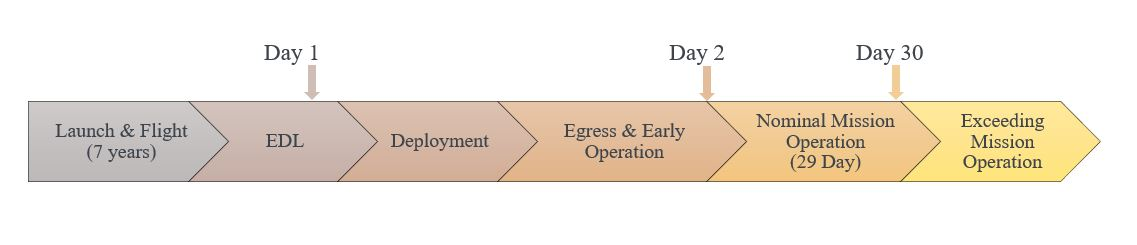
\includegraphics[width=1.0\textwidth]{Media/timeline}
\caption{Preliminary Mission Timeline for INSPIRE.}
\label{fig:timeline}
}
\end{figure}


Based on these missions phases some preliminary rover system modes as well as a basic mission timeline were concluded.

\subsection{Rover System Modes}
For this case study several rover system modes were defined. All ten modes are listed in \autoref{tab:systemmod}. 

They are seperated into two groups. The design critical modes are displayed in white and are defined as system modes, which significantly influence the preliminary design of the rover subsystem like the thermal or power subsystem. None design critical modes (grey) also have a major influence on multiple subsystems of the rover but play a secondary role in the thermal and power budget of the rover for this Phase 0 study. These non design critical modes extend from the rover storage and launch until the finale deployment of the rover is completed. These modes and their design options depend heavily on the final design of the lander with which INSPIRE flies to Europe. Therefore, a clear definition of such modes is not possible at this time in the course of this phase 0 study. However, the respective considerations, preferences and options have been briefly described in the mode descriptions. It is important to note that INSPIRE's goal is to provide a flexible rover design with as few hard requirements as possible for the parent lander. Therefore, many aspects of the rover, as well as the none design critical modes, will need to be further defined and elaborated in later phases of the project in close consultation with the customer. \\
For example, the exact interfaces between rover and lander should be defined in more detail. Depending on the subsequently chosen interfaces, many possibilities may arise in the corresponding rover system modes. With an appropriate interface, for example, the excess electrical and thermal energy of the RTG, which is already active during the flight, could be used to supply the lander system with heat and power. A corresponding interface could also enable the transmission of health checks from INSPIRE. \\
The deployment phase will strongly depend on the final design of the lander, INSPIRE's position within the lander and also the possibilities that the lander provides to INSPIRE.
Possible deployment strategies would be as follows:

\begin{itemize}
\itemsep0pt
\item	\textbf{Option 1:} If INSPIRE on ground level: Release from storage box through spring mechanism or actuators. Rover storage configuration allows rolling and possible motorized actuation
\item	\textbf{Option 2:} If INSPIRE is above ground level: Similar as Option 1 but an additonal ramp and ramp deployment would be required.
\item	\textbf{Option 3:} INSPIRE will be deployed through the landers robotic arm if it is capable of lifting its mass.
\end{itemize}


% Please add the following required packages to your document preamble:
% \usepackage{graphicx}
% \usepackage[table,xcdraw]{xcolor}
% If you use beamer only pass "xcolor=table" option, i.e. \documentclass[xcolor=table]{beamer}
\begin{table}[H]
\centering
\resizebox{\textwidth}{!}{%
\begin{tabular}{|c|c|c|l|}
\hline
Number & Rover System Modes                  & Abbrevation & \multicolumn{1}{c|}{Definition}                                                                                                                                                                                                                                                                                                                                                                                                                                                                                                                                                                                                   \\ \hline
\rowcolor[HTML]{C0C0C0} 
0      & Launch/Off Mode                     & OFF         & \begin{tabular}[c]{@{}l@{}}From Launch until EDL Phase\\ Rover System is OFF\\ Exact mode description t.b.d. and can be adapted to meet the lander demands\\ Health tests on Occasion during flight time are foreseen (PCDU could be active)\\ Batteries on Storage Capacity at launch and may be recharged on occasion (like Rosetta Mission)\\ Telemetry data shall be sent by the Lander (optional if possible)   \\ RTG on =\textgreater Electrical and Thermal Power may be used \\ (for Lander Power and Thermal Systems) or is disposed of by shunts\end{tabular}                                                          \\ \hline
\rowcolor[HTML]{C0C0C0} 
1      & Entry, Descent and Landing          & EDL         & \begin{tabular}[c]{@{}l@{}}From Entry until next morning after secure landing of Lander on Europa\\ See Mode OFF\\ PCDU ON after secure landing (Powered by RTG)\\ Heaters ON (powered by remaining RTG Power)\\ Battery charging if no Kill Switch is used\end{tabular}                                                                                                                                                                                                                                                                                                                                                          \\ \hline
\rowcolor[HTML]{C0C0C0} 
2      & Deployment and Early Operation Mode & EOP         & \begin{tabular}[c]{@{}l@{}}First Morning after EDL\\ Exact mode description t.b.d. and can be customized to lander \\ =\textgreater Dependant on final Lander Design\\ Critical Deployments (Egress System) and leaving the lander\\ Optional whether Kill Switch ejected =\textgreater Battery charging can start\\ Rover System Activation possibilities: Kill Switch, Lander Interface, HPC from Earth\\ PCDU ON\\ OBC ON\\ Heaters ON\\ After sufficient Battery Capacity is reached (50\%): Deployment of Rover Boogie \\ and checkout/health check of all Rover Systems\\ Afterward switching to Charging Mode\end{tabular} \\ \hline
3      & Idle/ Perception                    & ID          & \begin{tabular}[c]{@{}l@{}}During Idle Operation Time\\ Rover powered by RTG or Batteries (Excess Power charges Batteries)\\ PCDU ON\\ All Components in Standby or Power Saving Mode if possible\\ Stereovision Camera ON for Orientation and Observation (Science Data)\\ Hazcams and OBC ON for Orientation and Path Analysation\\ COMM ON for larger time intervals (Listening Mode)\end{tabular}                                                                                                                                                                                                                             \\ \hline
4      & Safe Mode/ Hibernation (SAFE)       & SAFE        & \begin{tabular}[c]{@{}l@{}}Entered in case of emergency or contingency Rover    \\ Survival Mode =\textgreater Minimum Power\\ PCDU ON  \\ COMM sends Emergency Signal then switches to\\ COMM ON for small time intervals (Listening Mode)\\ OBC OFF until Command received =\textgreater High Power Commands (HPC)\\ Heaters ON\\ Science data shall be stored without data loss\\ Applicable during Day and Nighttime\\ Exit after receiving the corresponding command\\ (Optional: Timer ON and Restart of Rover System after time period has passed)\end{tabular}                                                            \\ \hline
6      & Communication                       & COMM        & \begin{tabular}[c]{@{}l@{}}During Transmission of major Telemetry or Science Data\\ Rover powered by RTG or Batteries (Excess Power charges Batteries)\\ PCDU ON\\ All Components in Standby or Power Saving Mode if possible\\ OBC SB\\ COMM ON (Transmission Mode)\end{tabular}                                                                                                                                                                                                                                                                                                                                                 \\ \hline
7      & Charging                            & BAT         & \begin{tabular}[c]{@{}l@{}}For Battery charging\\ Rover batteries charged by RTG\\ PCDU ON\\ All Components in Standby or Power Saving Mode if possible\\ OBC SB\\ Quit after sufficient charge is reached\end{tabular}                                                                                                                                                                                                                                                                                                                                                                                                           \\ \hline
8      & Locomotion                          & LOC         & \begin{tabular}[c]{@{}l@{}}For Rover Movement and Observation\\ Locomotion and Navigation ON\\ Hazcams and Traversing Path Analysis ON\\ OBC ON\\ PCDU ON\\ COMM OFF\\ Stereovision Camera ON for Orientation and Observation (Science Data)\\ Only during Daytime\end{tabular}                                                                                                                                                                                                                                                                                                                                                   \\ \hline
9      & Payload Observation Mode            & OBS         & \begin{tabular}[c]{@{}l@{}}Payload Mode for Science Data Collection during Daytime\\ OBC ON\\ PCDU ON   \\ COMM OFF\\ Stereovision Camera ON for Orientation and Observation (Science Data)\\ RADAR ON for Ground Investigation =\textgreater Drill Location\\ Only during Daytime\end{tabular}                                                                                                                                                                                                                                                                                                                                   \\ \hline
10     & Payload: Ice Core Mode              & ICE         & \begin{tabular}[c]{@{}l@{}}Payload Mode for   Science Data Collection during Daytime or Nighttime\\ OBC ON\\ PCDU ON\\ COMM OFF\\ Ice Core Drill ON during Ice   Core Sample Collection\\ Afterwards Sample will be   analysed =\textgreater APXS ON\end{tabular}                                                                                                                                                                                                                                                                                                                                                                 \\ \hline
\end{tabular}%
}
\caption{Collection of Rover System Modes. [Kommt noch in Anhang]}
\label{tab:systemmod}
\end{table}
